\documentclass[conference,a4paper]{IEEEtran}

% Escritura mejorada de fórmulas matemáticas
\usepackage{amsmath}

% Inserción de gráficos
\usepackage{graphicx}

% Escritura de pseudocódigo
\usepackage[kw]{pseudo}

% Escritura mejorada de tablas
\usepackage{booktabs}

% Escritura mejorada de citas bibliográficas
\usepackage{cite}

% Inserción de enlaces
\usepackage{hyperref}

\usepackage{float}

\usepackage{titlesec}

\titlespacing*{\section}
{2pt}      % Sangría izquierda
{2pt}     % Espacio *antes* del título
{1pt}      % Espacio *después* del título

\titlespacing*{\subsection}
{2pt}{2pt}{1pt}

% Macros traducidas
\def\contentsname{Índice general}
\def\listfigurename{Índice de figuras}
\def\listtablename{Índice de tablas}
\def\refname{Referencias}
\def\indexname{Índice alfabético}
\def\figurename{Fig.}
\def\pseudoname{Pseudocodigo}
\def\tablename{TABLA}
\def\partname{Parte}
\def\appendixname{Apéndice}
\def\abstractname{Resumen}
% IEEE specific names
\def\IEEEkeywordsname{Palabras clave}
\def\IEEEproofname{Demostración}

\setlength{\parskip}{0.5em}

\begin{document}

\title{Desarrollo de un Agente Inteligente para Otelo basado en MCTS-UCT y Redes Neuronales}

\author{
  \IEEEauthorblockN{Nuno José del Pino Escalante}
  \IEEEauthorblockA{
    \textit{Dpto. Ciencias de la Computación e Inteligencia Artificial}\\
    \textit{Universidad de Sevilla}\\
    Sevilla, España\\
    nundelesc@alum.us.es}
  
  \and
  
  \IEEEauthorblockN{Javier Soria Blanco}
  \IEEEauthorblockA{
    \textit{Dpto. Ciencias de la Computación e Inteligencia Artificial}\\
    \textit{Universidad de Sevilla}\\
    Sevilla, España\\
    javsorbla@alum.us.es}
}

\maketitle


% Resumen
\begin{abstract}
  Este trabajo tiene como objetivo el desarrollo de un agente inteligente que sea capaz de jugar al juego Otelo 
  de manera óptima, es decir, siendo capaz de encontrar las mejores jugadas posibles en cada situación. Esto 
  se realizará mediante la aplicación del algoritmo de Monte Carlo Tree Search (MCTS), siguiendo Upper Confidence 
  Bound for Trees (UCT). Así mismo, se comparará la eficacia del agente usando una política de selección aleatoria, 
  frente al uso de una red neuronal para predecir la mejor acción posible.
  
  Los resultados obtenidos a lo largo de las pruebas realizadas evidencian la efectividad de un agente que implementa el algoritmo UCT, 
  así como el potencial que puede tener si se combina con una red neuronal entrenada adecuadamente.

\end{abstract}


% Palabras claves
\begin{IEEEkeywords}
  Inteligencia Artificial, Otelo, MCTS, UCT, Red Neuronal, Agente, Modelo.
\end{IEEEkeywords}


\section{Introducción}

Otelo es un juego de estrategia por turnos para dos jugadores, disputado en un tablero de 8×8 casillas. 
El objetivo consiste en capturar las fichas, o discos, del oponente, de modo que el ganador sea aquel que tenga más 
discos de su color en el tablero al finalizar la partida. Así mismo, solo se pueden realizar movimientos hacia casillas vacías 
y que, a su vez, impliquen la captura de discos del oponente, de tal manera que, si ninguno de los jugadores dispone de 
movimientos válidos, o si el tablero se llena por completo directamente, la partida se da por finalizada. A pesar de sus reglas sencillas, 
Otelo presenta un espacio de estados bastante complejo, lo que lo convierte en un entorno idóneo para el desarrollo y evaluación 
de algoritmos de inteligencia artificial.

A lo largo de los años, se han empleado diversas técnicas para desarrollar agentes capaces de jugar a juegos 
similares, destacando especialmente los enfoques que combinan métodos de búsqueda y aprendizaje profundo. 
Dos de los ejemplos más conocidos son los programas “AlphaGo”~\cite{b1} y “AlphaZero”~\cite{b2}, diseñados con propósitos similares 
a los de este trabajo, aunque orientados a juegos más complejos como el go, shogi y ajedrez.

El objetivo principal de este trabajo es demostrar que el uso de un algoritmo de búsqueda como \emph{Monte Carlo Tree Search} (MCTS) 
puede dar lugar a un agente competente en Otelo. Además, se pretende evaluar en qué medida una política basada en las predicciones 
de una red neuronal puede sustituir eficazmente a la política de selección aleatoria propia de UCT, mejorando así la calidad de las decisiones del agente. 
La principal contribución del trabajo consiste en una arquitectura funcional capaz de generar datos, entrenar modelos y refinar iterativamente el rendimiento del agente 
mediante ciclos de autoaprendizaje.

Inicialmente, se propone un diseño sencillo del agente basado únicamente en UCT para la toma de decisiones. Este primer agente será utilizado 
para generar un conjunto de datos con el que se entrenará una red neuronal que potenciará la toma de decisiones en el algoritmo. 
Posteriormente, se llevarán a cabo sucesivos ciclos de juego automático y reentrenamiento con el fin de incrementar progresivamente la eficacia y la habilidad del agente.

Este documento se organiza en seis secciones, incluyendo la presente introducción. En la Sección II se describen en mayor detalle las técnicas empleadas y se revisan algunos 
trabajos relacionados. En la Sección III se expone la metodología seguida y se detalla la implementación del sistema. La Sección IV está dedicada a los experimentos realizados 
y al análisis de los resultados obtenidos. En la Sección V se presentan las conclusiones del proyecto, así como posibles líneas futuras de mejora. Finalmente, en la sección VI 
se encuentra una declaración de uso de IA generativa. Al final del documento se incluyen las referencias bibliográficas utilizadas.

\section{Preliminares}

\subsection{Métodos empleados}

El desarrollo del agente propuesto se basa en la combinación de dos enfoques principales: el método de búsqueda \emph{Monte Carlo Tree Search} (MCTS), 
reforzado mediante la técnica \emph{Upper Confidence Bounds for Trees} (UCT), y una red neuronal entrenada mediante auto juego. 

A continuación, se detallan estos métodos y técnicas utilizados:

Se pueden usar listas por puntos como sigue:
\begin{itemize}
\item \emph{Monte Carlo Tree Search} (MCTS): Es un método de búsqueda que toma decisiones óptimas en dominios complejos mediante simulaciones aleatorias. Consiste en realizar exploraciones del espacio de decisiones, construyendo un árbol de búsqueda cuya expansión está guiada por los resultados obtenidos durante dichas simulaciones. Además, se trata de un algoritmo estadístico anytime, es decir, puede interrumpirse en cualquier momento y ofrecer una solución válida, mejorando progresivamente su rendimiento cuanto más tiempo de cómputo se le conceda. Además, su capacidad para operar con poco o ningún conocimiento específico del dominio lo hace particularmente atractivo en contextos como el de Otelo.
\item \emph{Upper Confidence Bounds for Trees} (UCT): Enfoque de MCTS en el que se guía la selección de nodos combinando la recompensa media obtenida con una estimación del potencial inexplorado del nodo. Proporciona un equilibrio entre explotación y exploración, lo que mejora significativamente la eficiencia del algoritmo. En concreto, cada vez que un nodo debe seleccionar uno de sus hijos, se aplica la fórmula UCB1 para calcular un valor asociado a cada acción posible. Esta fórmula combina la recompensa promedio estimada de esa acción (en la que se basa la explotación) con un término de exploración, proporcionando así el equilibrio mencionado. Además, garantiza que todas las acciones serán exploradas al menos una vez, y que las más exitosas tenderán a ser seleccionadas con mayor frecuencia. UCT se ha consolidado como una de las variantes más exitosas de MCTS, siendo utilizada como componente central en sistemas como AlphaGo y AlphaZero, mencionados anteriormente. Su simplicidad, eficiencia y capacidad de generalización lo convierten en una elección especialmente adecuada para entornos como Otelo.
\item Redes Neuronales Multicapa: Se utiliza una red neuronal de tipo \emph{feedforward} con varias capas ocultas, entrenada mediante aprendizaje automático supervisado, es decir, la salida pretendida del modelo para cada entrada de datos de entrenamiento es conocida, y se usa para evaluar las predicciones de la red~\cite{b3}. Este tipo de red permite aprender relaciones complejas entre entradas y salidas, transformando los datos progresivamente a través de capas interconectadas~\cite{b4}. En este proyecto, la red actúa como una política del agente, aprendiendo a predecir la posibilidad de victoria dado un estado del juego. Para ello, se entrena con datos recogidos en partidas generadas por el agente, sustituyendo así la política aleatoria por una basada en las predicciones de la red.
\end{itemize}

\subsection{Trabajo Relacionado}

Gran parte de este trabajo está basado en el artículo “A survey of Monte Carlo Tree Search Methods”~\cite{b5}, el cual ha proporcionado un entendimiento 
del funcionamiento y utilidad del algoritmo MCTS junto con UCT en el contexto de este trabajo. Así mismo, se ha usado tanto el pseudocódigo de UCT como 
las enseñanzas proporcionadas por este artículo para la implementación del agente inteligente.

Así mismo, como ya se ha mencionado anteriormente, existen aproximaciones similares para juegos más complejos de abordar computacionalmente. 
En concreto, los artículos sobre “AlphaGo”~\cite{b6} y “AlphaZero”~\cite{b7}, son bastante recomendables para aprender el impacto de un correcto uso del \emph{Deep Learning},
o aprendizaje profundo, en la búsqueda adversaria, permitiendo la creación de agentes sumamente hábiles en este tipo de juegos.

Por último, se hace especial mención a un proyecto reciente bastante similar a este~\cite{b8}, que también propone un agente inteligente capaz de jugar a Otelo, 
solo que utilizando otras técnicas como el algoritmo minimax y la poda alfa-beta.

\section{Metodología}

En primer lugar, se desarrolló un sistema con las reglas del juego, que permitiera jugar partidas de forma simple a través de la interfaz de línea de comandos, 
en la que se le pregunta al usuario por la jugada que desea realizar. Evidentemente, dado que no se había implementado el agente desde un principio, el usuario debía 
jugar contra sí mismo, algo más que suficiente para comprobar el correcto funcionamiento del juego, de tal manera que pudiera ser utilizado para la generación de 
datos de ejemplo a través de la simulación de partidas.

\begin{figure}[H]
  \centering
  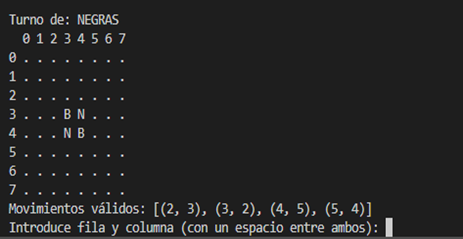
\includegraphics{interfaz}
  \caption{Interfaz del juego, mostrando el turno del jugador}
  \label{fig:interfaz}
\end{figure}

Posteriormente, se realizó la implementación del agente siguiendo el pseudocódigo proporcionado en el artículo sobre Monte Carlo mencionado anteriormente. 
Este agente actuó como punto de partida para simular las partidas que proporcionarían los datos de entrenamiento. Desde un nodo que representa el estado del tablero 
y el jugador activo en ese turno de la partida, realiza tantas simulaciones de la partida como se le indique mediante un parámetro, manteniendo un equilibrio entre exploración y 
explotación para la generación de un árbol de búsqueda. Una vez encontrado un nodo terminal, en el que la partida ha acabado, retropropaga 
el número de visitas de los distintos nodos, así como la recompensa, que va cambiando de signo para reflejar el cambio de perspectiva que 
sufre el juego al alternar turnos entre ambos jugadores, de tal manera que, si un resultado ha sido bueno para el jugador activo en un nodo,
habrá sido malo para el jugador del nodo padre. Este proceso se lleva a cabo de manera reiterada, de tal manera que, al terminar una iteración, 
se vuelva al nodo raíz para seguir expandiendo el árbol de búsqueda. Se realizarán tantas iteraciones como se indique, teniendo en cuenta que 
un mayor número de iteraciones aumenta la posibilidad de tomar una decisión óptima, pero que a su vez aumenta en gran medida el coste computacional y, 
en consecuencia, los tiempos de espera. Por esta razón, es importante encontrar un número de iteraciones que proporcione un balance adecuado 
entre ambos conceptos. Además, dada la simplicidad intencionada para esta primera versión del agente, utiliza una política de selección aleatoria, 
lo que hace que no siempre encuentre las jugadas óptimas, especialmente si el número de iteraciones no es suficiente para realizar una 
exploración del árbol suficiente. En concreto, el agente sigue el siguiente pseudocódigo:

\begin{figure}[H]
  \begin{pseudo}
    \textbf{Función UCTSEARCH}($s_0$) \\
    \> Crear nodo raíz $v_0$ con estado $s_0$ \\
    \> \textbf{Mientras} esté dentro del presupuesto computacional \\
    \> \> $v_i \leftarrow \text{TREEPOLICY}(v_0)$ \\
    \> \> $\Delta \leftarrow \text{DEFAULTPOLICY}(s(v_i))$ \\
    \> \> \text{BACKUP}$(v_i, \Delta)$ \\
    \> \textbf{Devolver} $a(\text{BESTCHILD}(v_0, 0))$ \\

    \\

    \textbf{Función TREEPOLICY}($v$) \\
    \> \textbf{Mientras} $v$ es no terminal \\
    \> \> \textbf{Si} $v$ no está totalmente expandido \\
    \> \> \> \textbf{Devolver} \text{EXPAND}($v$) \\
    \> \> \textbf{Sino} \\
    \> \> \> $v \leftarrow \text{BESTCHILD}(v, C_p)$ \\
    \> \textbf{Devolver} $v$ \\

    \\

    \textbf{Función EXPAND}($v$) \\
    \> Escoger $a \in$ acciones sin intentar de $A(s(v))$ \\
    \> Añadir nuevo hijo $v'$ a $v$ \\
    \> \> Con $s(v') = f(s(v), a)$ \\
    \> \> Y $a(v') = a$ \\
    \> \textbf{Devolver} $v'$ \\

    \\

    \textbf{Función BESTCHILD}($v, c$) \\
    \> \textbf{Devolver} $\displaystyle \arg\max_{v' \in \text{hijos de } v} \left( \frac{Q(v')}{N(v')} + c \sqrt{\frac{2 \ln N(v)}{N(v')}} \right)$ \\

    \\

    \textbf{Función DEFAULTPOLICY}($s$) \\
    \> \textbf{Mientras} $s$ no es terminal \\
    \> \> Escoger $a \in A(s)$ de manera \\
    \> \> uniformemente aleatoria \\
    \> \> $s \leftarrow f(s,a)$ \\
    \> \textbf{Devolver} recompensa para el estado $s$ \\

    \\

    \textbf{Función BACKUP}($v, \Delta$) \\
    \> \textbf{Mientras} $v$ es no nulo \\
    \> \> $N(v) \leftarrow N(v) + 1$ \\
    \> \> $Q(v) \leftarrow Q(v) + \Delta$ \\
    \> \> $\Delta \leftarrow -\Delta$ \\
    \> \> $v \leftarrow$ padre de $v$
  \end{pseudo}
  \label{pcd:uct}
\end{figure}

Donde v es un nodo del árbol, s(v) es el estado del tablero en ese nodo, Q(v) es la recompensa total de 
la simulación llegado ese nodo, N(v) es el número de veces que se ha visitado cada nodo, f(s, a) es la función 
que aplica la acción al estado s y c es el término de exploración, que corresponde al siguiente valor: $c = \frac{1}{\sqrt{2}}.$

Cabe destacar que la implementación de dicho algoritmo en código debe ser ajustada, ya que se deben tener en cuenta aquellos nodos 
en los que ninguna acción es posible para el jugador asociado, así como otros detalles causados por convenciones del lenguaje de 
programación en el que se trabaja, pero el núcleo del algoritmo no cambia.

Una vez implementado y comprobado el agente, se procede a la generación de datos para entrenar la red neuronal. Para ello, 
se simulan partidas en las que el agente juega contra sí mismo, de tal manera que tras cada acción se guarda el estado del tablero, 
que es etiquetado con –1, 0 o +1, en función de si el jugador activo en dicho estado perdió, empató o ganó la partida, respectivamente. 
Además, se incluye información de quién era dicho jugador, para que la red pueda interpretar correctamente los datos. Este conjunto 
de datos se convierte en un \emph{DataFrame} de \emph{Pandas}~\cite{b9}, y es almacenado en un archivo \emph{Pickle} (.pkl)~\cite{b10}, propio de Python y que se usa 
ya que permite convertir objetos de este lenguaje en formato binario de manera sencilla y rápida. En busca de menores tiempo de espera, 
se realiza el procedimiento de simulación de partidas de manera paralela, es decir, usando los distintos hilos de la CPU, se simularán tantas 
partidas como sea posible al mismo tiempo, juntando después los resultados y datos reunidos. Esto es posible gracias al módulo \emph{multiprocessing} 
de Python~\cite{b11}, a partir de la clase \emph{Pool}, que actúa como un administrador de distintos procesos que son lanzados, 
encargados de simular partidas a partir de los argumentos que reciben.

Para la generación de datos, se proponen distintos tipos de simulación de partidas, de tal manera que es posible simular partidas 
del agente jugando contra sí mismo, así como el agente enfrentándose a un oponente que escoge siempre movimientos aleatorios, 
y enfrentamientos entre el agente usando la política por defecto propia de UCT frente al agente que use una red neuronal entrenada 
como política. Para los 2 últimos casos, se incluye información de los resultados del agente, que son de interés conocer. Evidentemente, 
la generación de datos inicial será del agente jugando contra sí mismo, sin red neuronal, y estableciendo el número de partidas 
simuladas a 500, con 500 iteraciones del algoritmo, obteniendo así un conjunto de datos lo suficientemente amplio, asegurando que 
las decisiones tomadas, si bien no siempre son las óptimas, son suficientemente buenas y, en especial, rápidas.

Por otra parte, la red neuronal consiste en 6 capas, de tal manera que 4 de ellas son ocultas. En primer lugar, la capa de entrada es una convolucional de 2 dimensiones, 
compuesta por 128 filtros de tamaño 3x3 que sirve para detectar patrones espaciales simples del tablero. La siguiente capa es idéntica a la anterior, 
y tiene como objetivo aprender patrones más complejos, alcanzando un entendimiento aún mayor del juego. A continuación, hay una capa que convierte 
la salida tridimensional de la capa anterior a un vector unidimensional, de tal manera que pueda ser interpretada por capas posteriores. 
Dichas capas son 2 densas de 128 y 64 neuronas respectivamente, con función de activación ReLU, correspondiente a la ecuación~\eqref{eq:relu}, que devuelve 0 para 
todos los valores negativos, y crece linealmente para los positivos. Estas capas permiten alcanzar un entendimiento profundo de distintas representaciones 
de los estados tablero. Por último, la capa de salida también es densa, con una única neurona, y con función de activación tanh, correspondiente
a la ecuación~\eqref{eq:tanh}, de tal manera que devuelve un valor contenido en [-1, 1], que representa la probabilidad de victoria del jugador activo en un estado determinado.

\begin{equation}
  \label{eq:relu}
  ReLU(z) = max(0, z)
\end{equation}

\begin{equation}
  \label{eq:tanh}
  tanh(x) = \frac{e^x - e^{-x}}{e^x + e^{-x}}
\end{equation}

Para la creación y entrenamiento de la red se usa principalmente la biblioteca \emph{Keras}~\cite{b12}. En concreto, el procedimiento es el siguiente:  
Se convierten los datos a un tensor 3D, un tablero de 8x8 con 4 canales representando las distintas características de los estados. 
La red recibe esta entrada, así como el atributo que debe predecir, correspondiente en nuestro caso a la probabilidad de victoria del jugador 
que se ha pasado como parámetro para su entrenamiento. De esta manera, se puede proceder al entrenamiento, que se realiza con el 
optimizador \emph{Adam}~\cite{b13}, que define algunos valores importantes por defecto, como el factor de aprendizaje, aunque pueden ser modificados 
en cualquier momento. Además, se usa como función de pérdida el error cuadrático medio (MSE), correspondiente a la ecuación~\eqref{eq:mse}, y el error 
absoluto medio (MAE), equivalente a la ecuación~\eqref{eq:mae}, como métrica de monitorización del desempeño del modelo. 

\begin{equation}
  \label{eq:mse}
  MSE = \frac{1}{|D|} \sum_{(x,y) \in D} (y - \hat{y})^2
\end{equation}

\begin{equation}
  \label{eq:mae}
  MAE = \frac{1}{|D|} \sum_{(x,y) \in D} |y - \hat{y}|
\end{equation}

Además del entrenamiento, es necesario evaluar la precisión de las predicciones de la red neuronal, de tal manera que es necesario dividir 
los datos de prueba en 2 conjuntos, uno para cada propósito. Dicha división se realiza utilizando la herramienta \emph{Scikit Learn}~\cite{b14}. 
Finalmente, queda una división 80-20, siendo el conjunto de entrenamiento mayor por necesidad. Así mismo, el entrenamiento se realiza en 50 épocas, 
y se procesarán tanto los datos de prueba como los de entrenamiento en mini lotes de tamaño 128. En los casos en los que el conjunto de datos sea 
demasiado grande, se aumentará la configuración a 100 épocas y tamaño de 256 para los mini lotes. Toda la configuración mencionada proporciona un 
equilibrio entre coste computacional y eficacia de la red neuronal.

Una vez entrenada la red neuronal, se puede sustituir la función de política por defecto tradicional de UCT, de tal manera que ahora las 
recompensas de los nodos estarán determinadas por la predicción de victoria en un estado determinado para el jugador que debe tomar la decisión, 
es decir, para el jugador del nodo raíz. Evidentemente, cuánto más precisa sea la red al determinar la posibilidad de victoria, 
mejores decisiones tomará el algoritmo, de tal manera que, si la red no está lo suficientemente entrenada, no mejorará en gran medida a la política 
tradicional. Esto mismo se analizará con más detalle en el siguiente apartado.

Para que el agente pueda usar correctamente el modelo, se ha utilizado la herramienta \emph{TensorFlow}~\cite{b15}, muy ligada a \emph{Keras}. 
En concreto, lo que se hace es convertir la información necesaria a un tensor que se le pasa como entrada a la red neuronal 
para que pueda predecir la posibilidad de victoria del jugador desde ese estado de la partida. Es importante que siempre se 
le pase el jugador que debe tomar la decisión de mover, es decir, al que le correspondería realizar un movimiento en la partida real, 
que equivale al jugador asociado al nodo raíz del árbol. De lo contrario, la red no sería capaz de predecir desde la perspectiva 
correcta, llevando a jugadas ineficientes.

Tras implementar el agente con la red neuronal como política de selección, es de gran importancia realizar un reentrenamiento, es decir, simular aún más partidas 
para formar nuevos conjuntos de datos que sirvan para volver a entrenar la red neuronal, mejorando así su eficiencia. Para ello, se propone un entrenamiento escalonado, 
de tal manera que no se empiece a simular partidas del agente jugando contra sí mismo directamente, sino que antes pase por un procedimiento de entrenamiento a partir 
de partidas simuladas contra un oponente totalmente aleatorio y contra el propio agente, pero usando la política de selección anterior. Al realizar esto, la red neuronal 
va aprendiendo progresivamente al ser expuesta en primera instancia a estados del tablero a los que es menos común llegar, y que son posibles gracias a la falta de 
estrategia del oponente aleatorio. Sin embargo, es importante que los datos que se obtengan a partir de estas simulaciones no sean los únicos que se utilicen para entrenar 
la red, ya que esto provocaría que el agente solo sea capaz de jugar de manera correcta frente a oponentes de poco nivel. Por tanto, lo ideal es que se añadan estos datos 
a un conjunto ya existente. Por otra parte, también aprende al enfrentarse a un agente sin red neuronal, que puede llegar a realizar jugadas más eficientes mientras la red 
no es lo suficientemente buena. El conjunto de datos se extiende progresivamente a medida que se completa cada proceso de generación de datos, que será sobrescrito 
ocasionalmente para olvidar estados antiguos producidos por jugadas ineficientes que ya no serán de tanta utilidad.

Por último, una vez se haya pasado por el proceso anterior, se llega a la última parte del reentrenamiento, consistente en enfrentar al agente, 
con la red neuronal ya entrenada suficientemente, contra sí mismo. Para que esto sea posible, es necesario introducir algo de ruido en la selección 
de los mejores hijos de los nodos, ya que, en caso contrario, siempre se realizarían las mismas jugadas, llevando al mismo resultado en cada partida simulada. 
Esto se debe a que, al introducir la red, se sustituye la aleatoriedad de la política por defecto de UCT por unas predicciones que siempre van a ser 
valores muy similares para un mismo estado. Realmente, esto es algo positivo en la creación de un agente competente, pero para el entrenamiento supone una 
clara falta de variedad en los datos. Es por ello que se introduce este ruido únicamente cuando se están generando datos de prueba. En concreto, se introducirá 
un ruido gaussiano usando el módulo \emph{random}~\cite{b16}

Tras pasar por todo este procedimiento, el agente está listo para jugar contra humanos, de manera que se ofrecerá la oportunidad de 
jugar contra las dos versiones del agente, es decir, con ambas políticas. También se permitirá ajustar la habilidad del agente, es decir, 
establecer el presupuesto computacional del que dispondrá.

\section{Resultados}

A continuación, se detallarán los distintos experimentos realizados, que generalmente tendrán como objetivo determinar 
la eficacia y habilidad del agente con ambas políticas, comparando además el rendimiento de ambas y comprobar si introducir la red neuronal tiene un efecto positivo o negativo.

\subsection{Agente con política aleatoria frente a oponente aleatorio}

En este experimento se busca analizar la eficacia del agente antes de establecer la red neuronal como política por defecto, 
enfrentándolo con un oponente que realiza acciones puramente aleatorias, es decir, que no sigue ningún tipo de estrategia. 
Para ello, se reutiliza la función que permite simular partidas del agente frente a dicho oponente, indicando a través de parámetros 
que se debe utilizar la política mencionada. Por cada partida simulada se muestra por pantalla el resultado de la partida, y una vez 
finalicen todas las partidas, se cuentan automáticamente todas las partidas ganadas y se calcula el porcentaje de victorias, 
que será la métrica que usaremos para el análisis. 

En concreto, se realizarán dos pruebas para la comparación, estableciendo los siguientes parámetros para cada una de ellas:

1)	Iteraciones del algoritmo: 500. Partidas jugadas: 500.

2)	Iteraciones del algoritmo: 1000. Partidas jugadas: 500.

Tras realizar las pruebas se obtienen los siguientes resultados: Para la primera prueba, se ganan 304 partidas, con un porcentaje de victorias del 60.8\%. 
Por otro lado, para la segunda prueba se obtienen 375 victorias, llevando a un porcentaje de victorias del 75\%.

A partir de estos resultados podemos obtener varias conclusiones. En primer lugar, resulta evidente que el agente sigue una estrategia que le permite ganar la mayoría 
de las veces contra un oponente de bajo nivel. Sin embargo, para que sea verdaderamente efectivo, necesita un presupuesto computacional suficientemente alto 
que le permita encontrar las mejores jugadas posibles, algo que se ve claro en la diferencia en el porcentaje de victorias al duplicar el número de iteraciones 
que se realiza en la búsqueda por árbol. 

Con estos resultados, podemos asumir con seguridad que el agente tiene potencial para ser habilidoso, siempre y cuando disponga de suficientes recursos. 
No obstante, estas simulaciones son frente a un oponente muy débil, que no sigue ningún tipo de estrategia. Al enfrentarse a un oponente humano, 
el porcentaje de victorias será menor, aunque dependiendo del nivel del jugador, el agente puede seguir obteniendo un número aceptable de victorias. 
En general, podemos estimar que, dada la implementación actual, el agente tiene el nivel de un jugador promedio de Otelo. Si bien podría ser mucho más habilidoso 
con un gran número de iteraciones sobre el algoritmo de búsqueda, esto no sería aceptable para enfrentarse a humanos dados los altos tiempos de espera que supondría.

El resultado no es excelente, pero lo suficientemente bueno como para que solo sean necesarias pequeñas modificaciones y optimizaciones 
para obtener un agente mucho más habilidoso, demostrando así que la aplicación del algoritmo UCT tiene mucho potencial para este juego.

\subsection{Calidad de la red neuronal}

Para este experimento, se realizarán distintas pruebas que determinarán la calidad de diversos aspectos de la red neuronal. 
Dichas pruebas están configuradas para realizarse tras cada entrenamiento realizado, aunque únicamente se mostrarán los del último, 
ya que a partir de ellos se podrá analizar la última versión de la red neuronal.

Es importante recordar los parámetros de entrenamiento que ya se habían mencionado anteriormente, es decir, un 20\% 
del contenido del conjunto de datos de entrenamiento para la evaluación, que se realiza en mini lotes de tamaño 128.

La evaluación se realiza a través de 3 métricas: Error cuadrático medio (MSE), error absoluto medio (MAE), y coeficiente de variación ($R^2$), correspondiente a la ecuación~\eqref{eq:r2}. 

\begin{equation}
  \label{eq:r2}
  R^2 = 1 - \frac{\mathrm{MSE}}{\mathrm{VAR}(D)}
\end{equation}

Para las 2 primeras métricas, cuanto menor sea el valor, mejores serán las predicciones de la red. Por otro lado, 
para la tercera métrica, el valor será mejor cuanto más cercano sea a 1, y si es cercano o incluso menor a 0, la red 
no es nada acertada. Pondremos un mayor énfasis en esta tercera métrica, ya que es la que mide en qué medida la 
varianza de los datos es explicada por la red neuronal. Las otras 2 son algo más sencillas de entender, simplemente 
miden el error medio de las predicciones, solo que el MSE castiga más los errores grandes, algo raro en este contexto 
ya que tanto las predicciones como los valores objetivos están en el rango [-1, 1].

Tras realizar las pruebas, se obtienen los siguientes valores: MSE = 0.2825, MAE = 0.2020, $R^2$ = 0.7099.

De estos resultados podemos afirmar que la red neuronal es capaz de predecir acertadamente la mayoría de los valores, aunque todavía 
se podría refinar algo más. Un coeficiente de variación de 0.7099 no es malo en absoluto, pero podría ser mejor e índica que en situaciones 
reales pueda realizar predicciones desacertadas. Por otro lado, ambos errores son pequeños, aunque lo ideal sería que fueran aún menores, 
especialmente porque el rango de valores ya era pequeño de por sí.

En resumen, si bien la red neuronal podría refinarse aún más, parece ser lo suficientemente buena. Por otra parte, esto no 
indica que vaya a mejorar la política anterior, ya que cabe la posibilidad de que aún no haya comprendido del todo bien los 
distintos patrones y estados del tablero. Esto se evaluará en el siguiente experimento.

\subsection{Agente con red neuronal frente a agente sin red neuronal}

Ahora se busca analizar el impacto de usar una red neuronal para predecir las recompensas en la política por defecto del algoritmo. 
Para ello, reutilizamos la función que permite simular partidas entre los agentes de esta manera. En esta ocasión, se medirá el porcentaje de victorias 
del agente que implementa red neuronal, siguiendo exactamente el mismo procedimiento que en el primer experimento. Se realizarán tres pruebas distintas:

1)	Iteraciones del algoritmo: 500 para ambos agentes. Partidas jugadas: 500.

2)	Iteraciones del algoritmo: 1000 para ambos agentes. Partidas jugadas: 500.

3)	Iteraciones del algoritmo: 2000 para ambos agentes. Partidas jugadas: 100

Salta a la vista que la configuración es muy similar a la primera. Sin embargo, lo que se busca medir esta vez es distinto, ya que es interesante 
analizar la importancia del presupuesto computacional que se le ofrece a los agentes y determinar cuál de los dos se ve más beneficiado por un mayor valor. 
Por esa razón, se incluye una tercera prueba, de dimensiones menores en cuanto a partidas jugadas, pero con un alto número de iteraciones.

Una vez realizadas las pruebas, se obtienen los siguientes resultados: Para la primera prueba, el agente con red neuronal gana un total de 128 partidas, 
es decir, un 37.8\% de victorias. Por otro lado, en la segunda prueba mejora, consiguiendo ganar 238 partidas, y obteniendo así un 47.6\% de victorias.
Para la última prueba, gana 51 partidas y, en consecuencia, obtiene un 51\% de victorias.

Los resultados implican que el agente que implementa la red neuronal es, en general, menos habilidoso, a partir de lo cual se puede concluir que 
la red no ha tenido un efecto positivo en cuanto a efectividad y toma de decisiones. Esto se puede deber a muchos motivos, pero el principal es 
la falta de entrenamiento de la red. Si bien era capaz de predecir correctamente los valores esperados en la evaluación en el experimento anterior, 
todo parece indicar que todavía no tiene un entendimiento profundo del juego, y que necesita ser entrenada con datos de prueba más abundantes y de 
mayor calidad para así poder realizar predicciones aún más precisas, asegurando una toma de decisiones más acertada. 

También es interesante analizar la diferencia en el porcentaje de victorias al aumentar el número de iteraciones del algoritmo. Dados los resultados, 
parece que el agente con red mejora en mayor medida que el anterior cuanto mayor presupuesto computacional se le ofrece. Esto se demuestra en la tercera 
prueba, en la que consigue superar por un pequeño margen al otro agente, aunque al haberse simulado menos partidas, los resultados no son tan significativos. 
Aun así, podemos concluir que con suficientes iteraciones puede igualar e incluso superar al agente anterior, aunque a efectos prácticos no sería viable 
debido al tiempo que le llevaría tomar una decisión.

A pesar de los resultados, cabe destacar que el uso de la red hace que el agente sea algo más eficiente en términos de tiempo, 
incluso si es afectado por un mínimo retraso inicial causado por la carga del modelo predictivo. Por tanto, si se consigue una red neuronal lo suficientemente buena, 
el agente no solo mejoraría en términos de habilidad sino también en tiempos. Por esta razón, a pesar de estos malos resultados, podemos afirmar que este enfoque 
tiene un gran potencial para construir un agente aún mejor, y para ello solo necesita más rondas de reentrenamiento, esta vez con partidas de mayor calidad.

Por último, todo esto no quiere decir que el agente que implementa una red neuronal es totalmente incompetente, ya que sigue siendo capaz de hacer jugadas decentes, 
especialmente cuando se establece un número alto de iteraciones para el algoritmo de búsqueda. Simplemente es peor que cuando se usaba la política por defecto propia de UCT. 
En general, podemos asumir con seguridad que, al menos, es mejor que un agente sin ningún tipo de estrategia, o con una estrategia extremadamente simple.

\section{Conclusiones}

En este trabajo se ha diseñado y desarrollado un agente capaz de jugar al Otelo utilizando dos políticas distintas para el algoritmo UCT. 
Una de ellas es la del propio algoritmo y otra se basa en las predicciones de una red neuronal entrenada para tales efectos. Además, 
se realizaron distintos experimentos para evaluar la eficacia de ambas, en los que se obtuvieron buenos resultados para la política 
tradicional de UCT. Por otro lado, la red neuronal obtuvo resultados decentes, aunque no puede decir lo mismo para la política que la toma como base.

En general, los resultados muestran que el agente con la política por defecto de UCT es bastante competente, llegando al nivel de jugadores promedios de Otelo, 
ya que es capaz de seguir una estrategia determinada y derrotar en la mayoría de ocasiones a un oponente débil. Por otra parte, la red neuronal demostró ser 
capaz de predecir resultados de las partidas con un nivel razonable de precisión, obteniendo errores bajos y demostrando tener un coeficiente de variación más que aceptable. 
Sin embargo, al integrar la red neuronal como nueva política por defecto, los resultados fueron algo decepcionantes, ya que no mostró una mejoría respecto a la política anterior.

En conclusión, tras comparar los resultados de ambas políticas, podemos determinar que la red neuronal todavía no es capaz de entender por completo el juego, 
de manera que sus predicciones no ayudan en gran medida a mejorar a la política anterior en cuanto a calidad de las decisiones. No obstante, se pueden sacar 
muchas conclusiones positivas de los resultados obtenidos. Por un lado, el agente basado totalmente en el algoritmo UCT es sólido y tiene potencial para mejorar. 
Además, con un entrenamiento más extenso y de mejor calidad para la red neuronal, es plausible que se logren no solo decisiones más acertadas, sino también una 
reducción en el tiempo de respuesta del agente sin sacrificar su habilidad, lo que evidencia un gran potencial para este enfoque, tal como se buscaba en este trabajo. 
Si bien el agente con red neuronal solo es suficientemente bueno cuando dispone de muchos recursos computacionales, en un futuro podría llegar a ser más hábil con pocos de esos recursos.

Para finalizar, se identifican diversas líneas de mejora y trabajo futuro. La más evidente es optimizar el entrenamiento y la arquitectura de la red neuronal, 
por ejemplo, incorporando capas convolucionales o densas adicionales, así como capas de normalización para mejorar la generalización. Así mismo, se propone explorar 
estrategias híbridas que combinen la simulación de UCT junto con predicciones precisas de una red neuronal, guiando así el proceso de selección, e incluso se podría 
mantener algo de la aleatoriedad propia de UCT. También es muy interesante la opción de mantener el árbol de búsqueda en caché, para así poder reutilizarlo en caso 
de que el adversario haga algún movimiento que lleve a alguno de los nodos explorados. De esta manera, se podría reducir el tiempo de respuesta y mejorar la calidad 
de las decisiones del agente, sin importar la política por defecto utilizada.

\section{Declaración de Uso de IA Generativa}

A lo largo de este proyecto, se ha hecho uso de inteligencia artificial generativa como apoyo para plantear ciertas partes de la implementación o resolver problemas surgidos 
durante la documentación. En concreto, se ha usado \emph{ChatGPT}, de \emph{OpenAI}. A continuación, se describen los aspectos en los que se ha usado, así como las entradas proporcionadas a los mismos.

\begin{itemize}
\item Almacenamiento de datos obtenidos en las simulaciones de partidas: Tras implementar el sistema de generación de datos, necesitábamos un formato de fichero en el que guardarlo, distinto a CSV, el cual se había usado con frecuencia en las prácticas del curso, ya que el formato de los datos era demasiado complejo. Para resolver la duda, se le proporcionó a la inteligencia artificial contexto sobre el formato de los datos, pidiendo que diera opciones y analizara ventajas y desventajas. Finalmente, nos decantamos por \emph{Pickle} por su sencillez de almacenamiento y carga de datos a través de \emph{Pandas}.
\item Paralelización de la simulación de partidas: Una vez llegado el momento de generar datos para entrenar la red neuronal, se percibió que el proceso era demasiado lento. Gracias a los conocimientos de asignaturas anteriores, sabíamos que una solución fácil era paralelizar el proceso, pero no recordábamos como hacerlo exactamente. Por tanto, se le preguntó a la inteligencia artificial que nos explicara una forma de conseguir simular varias partidas al mismo tiempo aprovechando los hilos del procesador. Usando la respuesta proporcionada y la documentación oficial de Python se llegó a una solución.
\item Documentación en LaTeX~\cite{b17}: Casi la totalidad del documento se pudo escribir sin problemas siguiendo la plantilla proporcionada. Sin embargo, se encontraron algunos problemas en tres aspectos: Las figuras no siempre aparecían en el lugar deseado, el pseudocódigo era difícil de escribir en este formato dados nuestros escasos conocimientos, y se desconocía la forma de convertir a formato PDF. Ante esto, se decidió pedir consejo a la inteligencia artificial, describiendo la fuente del problema y pidiendo soluciones viables. Como respuesta, se recibió una forma de forzar que las figuras se muestren donde deben, así como algunas formas de cambiar la separación entre párrafos y secciones para que las figuras se acabaran mostrando en el mismo lugar que en el formato \emph{Word}. También se recibió un prototipo de pseudocódigo que después fue modificado para ajustarlo a nuestras necesidades y se nos dio opciones de distintos sistemas para instalar que permitirían, entre otras cosas, la generación del documento PDF a través de líneas de comando.
\end{itemize}

\begin{thebibliography}{00}
\bibitem{b1} \href{https://deepmind.google/research/projects/alphago/}{Página web oficial del proyecto de investigación AlphaGo}, realizado por Google DeepMind.
\bibitem{b2} David Silver, Thomas Hubert, Julian Schrittwieser, Demis Hassabis: \href{https://deepmind.google/discover/blog/alphazero-shedding-new-light-on-chess-shogi-and-go/}{Entrada de blog divulgativa sobre AlphaZero}, desarrollado por Google DeepMind.
\bibitem{b3} \href{https://www.cs.us.es/docencia/aulavirtual/pluginfile.php/9264/mod_resource/content/5/Aprendizaje_automático_%28Contenido_teórico%29.pdf}{Apuntes de aprendizaje automático} de la asignatura Inteligencia Artificial, del Departamento de Ciencias de la Computación e Inteligencia Artificial, de la Universidad de Sevilla.
\bibitem{b4} \href{https://www.cs.us.es/docencia/aulavirtual/pluginfile.php/9479/mod_resource/content/2/Redes_neuronales_%28Contenido_teórico%29.pdf}{Apuntes de redes neuronales} de la asignatura Inteligencia Artificial, del Departamento de Ciencias de la Computación e Inteligencia Artificial, de la Universidad de Sevilla.
\bibitem{b5} C. B. Browne, E. Powley, D. Whitehouse, S. M. Lucas, P. I. Cowling, P. Rohlfshagen, S. Tavener, D. Perez, S. Samothrakis, and S. Colton, “A Survey of Monte Carlo Tree Search Methods,” IEEE Transactions on Computational Intelligence and AI in Games, vol. 4, no. 1, pp. 1–43, 2012, doi: \href{https://ieeexplore.ieee.org/document/6145622}{10.1109/TCIAIG.2012.2186810.}
\bibitem{b6} D. Silver, A. Huang, C. J. Maddison, A. Guez, L. Sifre, G. van den Driessche, J. Schrittwieser, I. Antonoglou, V. Panneershelvam, M. Lanctot, S. Dieleman, D. Grewe, J. Nham, N. Kalchbrenner, I. Sutskever, T. Lillicrap, M. Leach, K. Kavukcuoglu, T. Graepel, and D. Hassabis, “Mastering the game of Go with deep neural networks and tree search,” Nature, vol. 529, no. 7587, pp. 484–489, 2016, doi: \href{https://www.nature.com/articles/nature16961}{10.1038/nature16961.}
\bibitem{b7} D. Silver, J. Schrittwieser, K. Simonyan, I. Antonoglou, A. Huang, A. Guez, T. Hubert, L. Baker, M. Lai, A. Bolton, Y. Chen, T. Lillicrap, F. Hui, L. Sifre, G. van den Driessche, T. Graepel, and D. Hassabis, “Mastering the game of Go, Chess, and Shogi by self-play with a general reinforcement learning algorithm,” arXiv preprint, arXiv:1712.01815, 2017. \href{https://arxiv.org/abs/1712.01815}{arXiv:1712.01815}.
\bibitem{b8} Sandra Alegría Ocampo, de la Universidad de Cantabria: \href{https://repositorio.unican.es/xmlui/bitstream/handle/10902/33691/AlegriaOcampoSandra.pdf}{“Jugando al Othello con Inteligencia Artificial”.}
\bibitem{b9} \href{https://pandas.pydata.org/}{Página web oficial de Pandas.}
\bibitem{b10} \href{https://docs.python.org/3/library/pickle.html}{Documentación de Python sobre el módulo Pickle.}
\bibitem{b11} \href{https://docs.python.org/3/library/multiprocessing.html}{Documentación de Python sobre el módulo multiprocessing.}
\bibitem{b12} \href{https://keras.io/}{Página web oficial de Keras.}
\bibitem{b13} \href{https://keras.io/api/optimizers/adam/}{Página web de Keras con información de uso del optimizador Adam.}
\bibitem{b14} \href{https://scikit-learn.org/stable/}{Página web oficial de Scikit Learn.}
\bibitem{b15} \href{https://www.tensorflow.org/}{Página web oficial de TensorFlow.}
\bibitem{b16} \href{https://docs.python.org/3/library/random.html}{Documentación de Python sobre el módulo random.}
\bibitem{b17} \href{https://www.latex-project.org}{Página web oficial del sistema LaTeX.}
\end{thebibliography}


\end{document}
